% vim:sw=4:ts=4:autoindent:tw=72
% vim:sw=4:ts=4:autoindent:tw=72
\documentclass[a4paper,11pt]{report}
\usepackage[utf8]{inputenc}
\usepackage[T1]{fontenc}
\usepackage[usenames, dvipsnames]{color}
\usepackage[english]{babel}
\usepackage{amsmath,bm}
\usepackage{empheq} % rutor runt ekv
\numberwithin{equation}{chapter} 
\renewcommand{\frac}[2]{\dfrac{#1}{#2}}
\usepackage{units}
\usepackage{graphicx}
\graphicspath{{images/}}
\usepackage{bbm}
\usepackage{rotating}
\usepackage{icomma}
\usepackage{comment}
\usepackage{booktabs}
\usepackage{dsfont}
\usepackage{float}
\usepackage{subfigure}
\usepackage[a4paper, margin=3cm]{geometry}
\usepackage[font={small,it}]{caption}
\usepackage{t1enc}
\usepackage{amssymb}
\usepackage{url}
\usepackage{multicol}
\usepackage{wrapfig}
\usepackage{adjustbox}
\usepackage{wallpaper}
\usepackage[sorting=none,natbib=true,url=true]{biblatex}
\bibliography{references}
\usepackage{tabu} % använd "tabu" istället för "tabular"
\usepackage{longtable}
\usepackage{blindtext}
\usepackage{parskip}

% Typografiska rådet
% 2) 1.5 radavstånd (även om det står 1.3)
\linespread{1.3}
\usepackage[para,bottom]{footmisc}
\usepackage{hyperref}

\usepackage{appendix}

\usepackage{gensymb} 

% för sidhuvud
\usepackage{fancyhdr}
\fancypagestyle{plain}{
    \fancyhf{} % empty header and footer
    \renewcommand{\headrulewidth}{0pt} % ho header line
    \renewcommand{\footrulewidth}{0pt}% not footer line
    \fancyfoot[C]{\thepage}% like fancy style
}

% För kod
\usepackage{minted}
\newcommand{\code}[1]{\texttt{#1}}
\renewcommand\listingscaption{Lista}
\newcommand{\sgn}{\operatorname{sgn}}

% kommandon för att referera, använd dessa istället för \ref
\newcommand{\Tblref}[1]{Table~\ref{#1}}
\newcommand{\Figref}[1]{Figure~\ref{#1}}
\newcommand{\Secref}[1]{Section \ref{#1}~\emph{\nameref{#1}}}
\newcommand{\Chapref}[1]{Chapter \ref{#1}~\emph{\nameref{#1}}}
\newcommand{\Listref}[1]{List~\ref{#1}}
\newcommand{\tblref}[1]{table~\ref{#1}}
\newcommand{\figref}[1]{figure~\ref{#1}}
\newcommand{\secref}[1]{section \ref{#1}~\emph{\nameref{#1}}}
\newcommand{\chapref}[1]{chapter \ref{#1}~\emph{\nameref{#1}}}
\newcommand{\eqnref}[1]{(\ref{#1})}
\newcommand{\listref}[1]{list~\ref{#1}}

\newcommand*{\figuretitle}[1]{%
    {\centering
    #1
    \par\medskip}
}

% T0DO-kommando:
\newcommand{\todo}[1]{%
	\textbf{{\color{red} TODO: #1}}
}

% titeln på arbetet
\newcommand{\thesistitle}{Revealing relations in highly dimensional temporal data}
\newcommand{\thesissubtitle}{}


% var och när detta arbete gjordes
\newcommand{\whereandwhen}{%
	Department of Physics\\
	\textsc{Chalmers University of Technology}\\
	Göteborg, Sweden 2017\\
}

% vad är det för arbete?
\newcommand{\whatthisis}{%
	Master's thesis
}

\usepackage{pgfgantt} % För att göra Gantt-tabell
\usepackage{pdfpages} % för att inkludera pdf-fil

\begin{document}

\pagestyle{empty}
% vim:sw=4:ts=4:autoindent:tw=72
% Framsida
% OBS skilj på titelsida och framsida! se
% https://student.portal.chalmers.se/sv/chalmersstudier/kandidat-och-examensarbete/examensarbete/Sidor/utformning-rapporter-exjobb-kand.aspx

% från
% http://tex.stackexchange.com/questions/46280/how-to-create-a-background-image-on-title-page-with-latex
\ThisLRCornerWallPaper{1}{front_page.pdf}
\vspace*{3cm}
\begin{comment}
\begin{figure}[H]
\centering
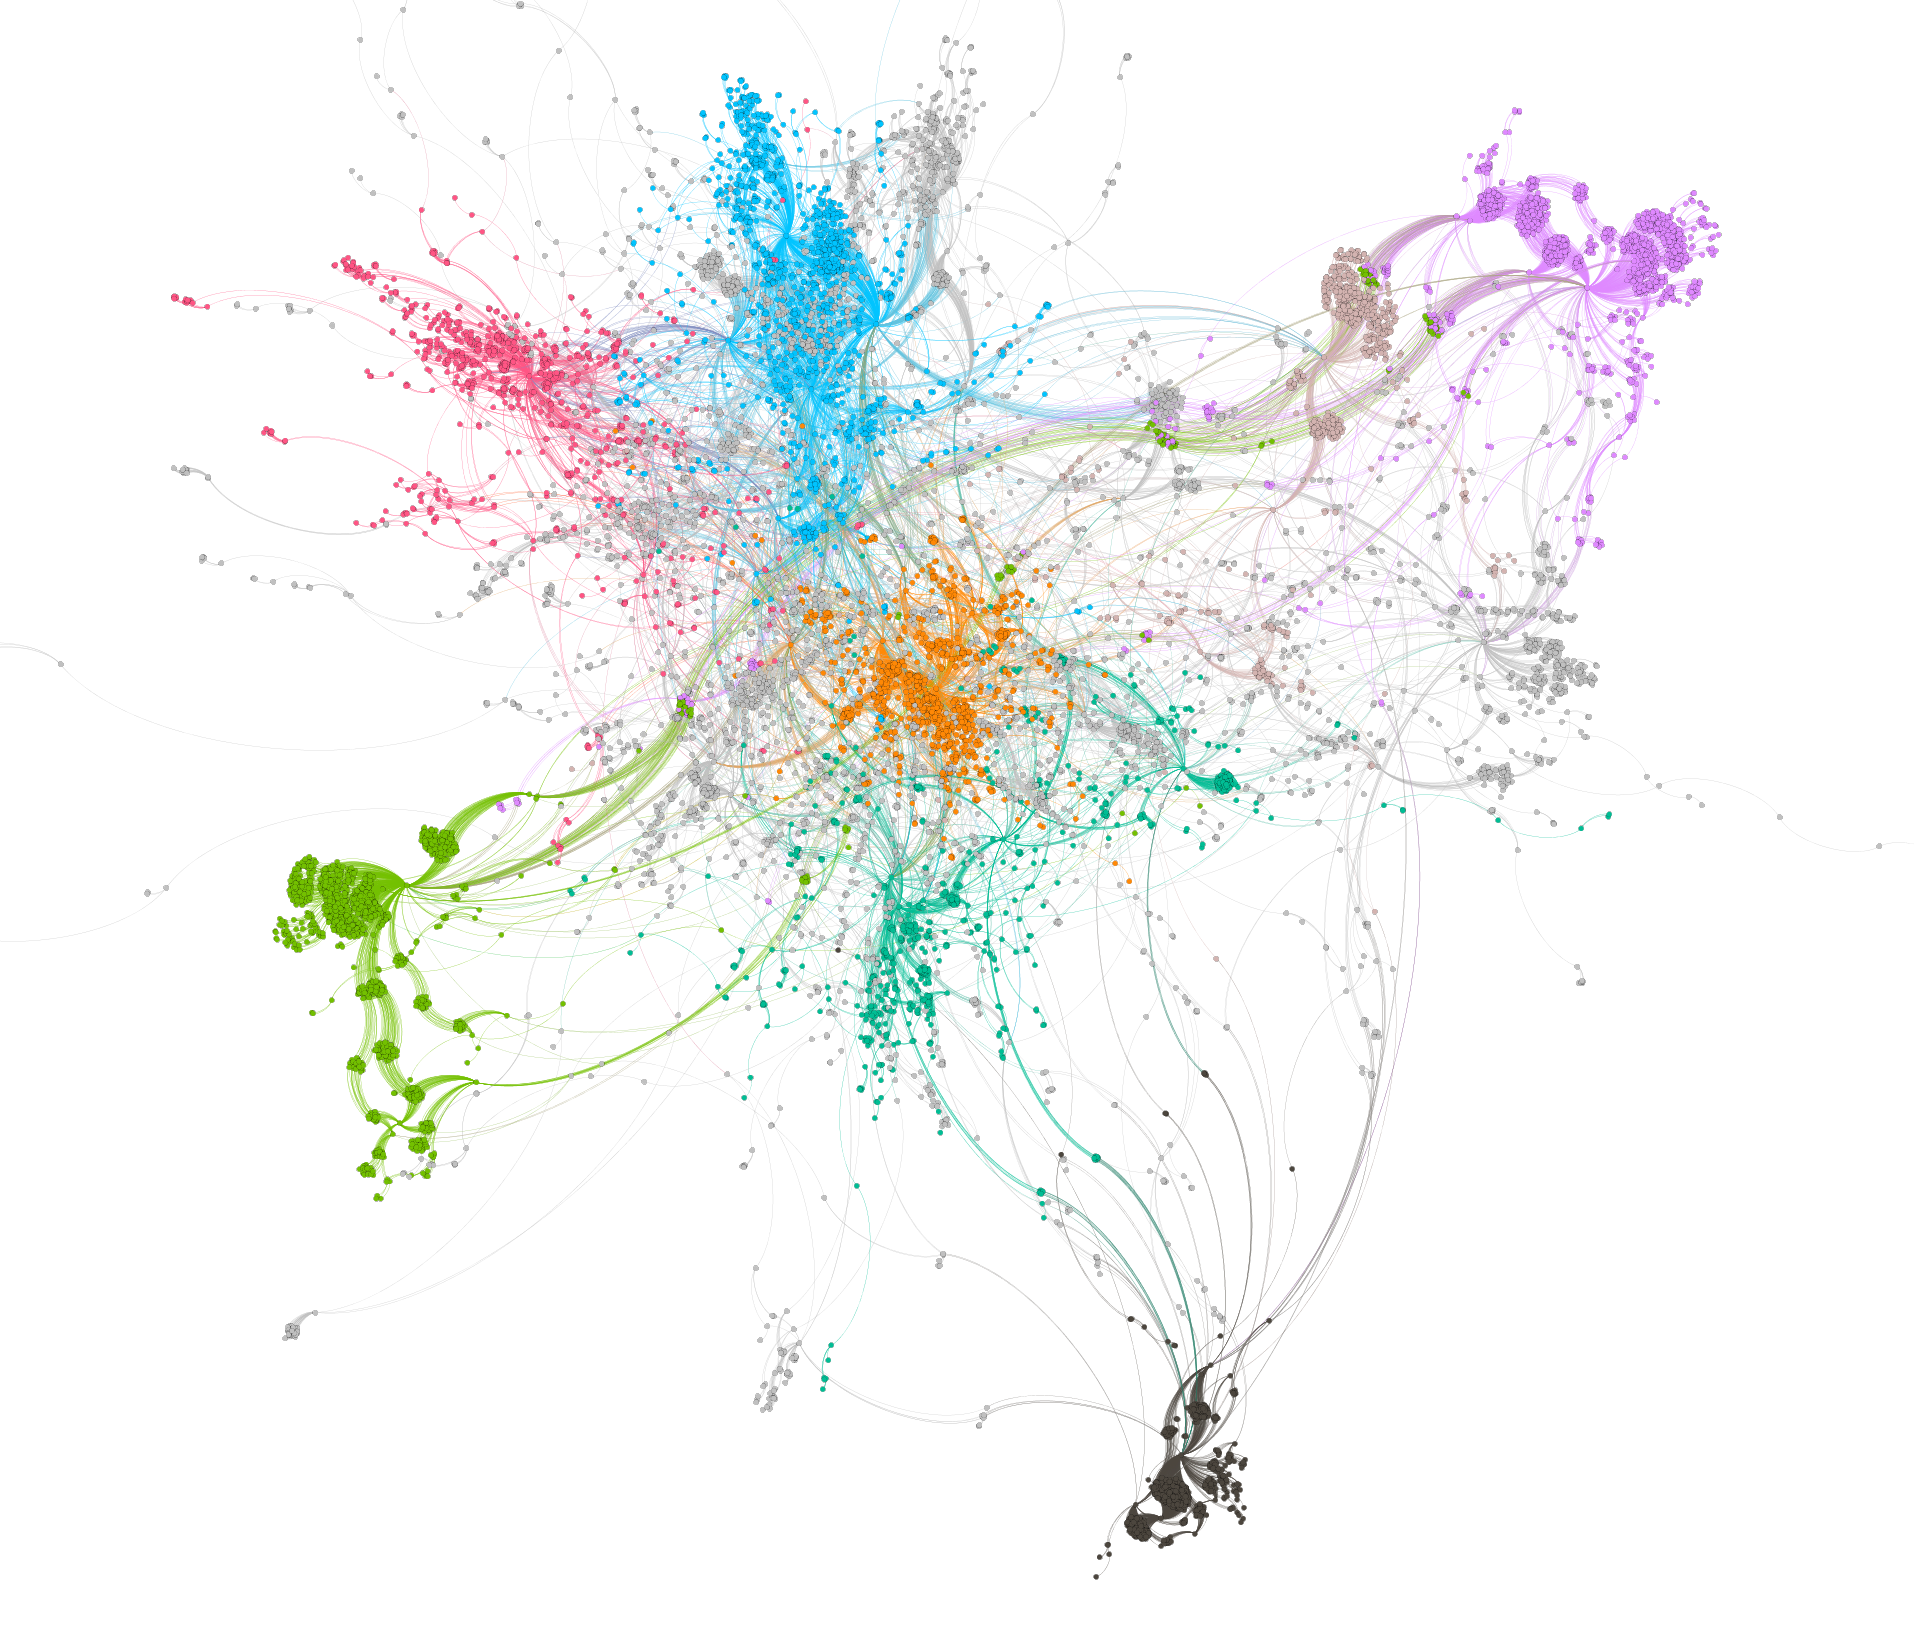
\includegraphics[width = 0.95\textwidth]{network.png}
\end{figure}
%\vspace*{\fill}
\begin{flushleft}
        \noindent{%
			% arbetstitel
			{\Huge \thesistitle} \\[.1cm]
			% undertitel

        	{\large \whatthisis}\\
        
			\bigskip
			\Large{%
				Henrik Adolfsson\\
				Josephine Cuellar Andersson\\
			}

		}
\end{flushleft}
\end{comment}

\thispagestyle{empty}
\newpage

\newpage
% vim:sw=4:ts=4:autoindent:tw=72
% Tryckortssida

\noindent
\thesistitle \\
\thesissubtitle \\
\whatthisis \\
\\
\large{%
    Henrik Adolfsson\\
	Josephine Cuellar Andersson\\
}

\vspace*{\fill}
\noindent
Image on front page:\\
Network of...

\thispagestyle{empty}
\newpage

% vim:sw=4:ts=4:autoindent:tw=72
% Titelsida
% OBS skilj på titelsida och framsida! se
% https://student.portal.chalmers.se/sv/chalmersstudier/kandidat-och-examensarbete/examensarbete/Sidor/utformning-rapporter-exjobb-kand.aspx

\begin{center}
	%\LARGE \textsc{Slutrapport}\\
	\bigskip
	\bigskip
	\Huge{Revealing relations in high \\dimensional data}\\
	\medskip
	\Large{-- BASED ON LINK PREDICTION AND NODE SIMILARITY \\IN A GRAPH} \\
\end{center}

\bigskip
\bigskip
\noindent\rule{\linewidth}{0.4pt}
\bigskip

% Taget från
% http://tex.stackexchange.com/questions/56875/how-do-i-make-one-minipage-the-same-size-as-another
\newlength\myheight
\begin{center}
	\begin{adjustbox}{%
		minipage=[t]{0.40\linewidth},
		gstore totalheight=\myheight
	}
		\begin{flushleft}
			% Namnen sorterade efter efternamn
			\large \emph{Authors:}\\
			Henrik Adolfsson\\
			\text{henado@student.chalmers.se}\\[0.3cm]
			Josephine Cuellar Andersson\\
			\text{josander@student.chalmers.se}\\[0.3cm] 
		\end{flushleft}
	\end{adjustbox}
	\hspace{0.5cm}
	\begin{adjustbox}{minipage=[t][\myheight]{0.4\linewidth}}
		\begin{flushright} \large
			\emph{Examiner:} \\
			Mats Granath\\ [0.3cm]

			\emph{Supervisors:} \\
			Staffan Truv\'e\\
			Michel Edkrantz\\
		\end{flushright}
	\end{adjustbox}
\end{center}

\vspace*{\fill}

\begin{center}
	\Large{%
		\whereandwhen
	}
\end{center}


\thispagestyle{empty}
\newpage


%%%%%%%%%%%%%%%%%%%%%%%%%%%%%%%%%%%%%%%%%%%%%%%%%%%%%%%%%%%%%%%%
% Front matter
\setcounter{page}{1}
\pagenumbering{roman}

% abstract
% vim:sw=4:ts=4:autoindent:tw=72

\noindent
\thesistitle\\
\thesissubtitle\\
\whatthisis\\
\\
\large{%
    Henrik Adolfsson\\
	Josephine Cuellar Andersson\\
}\\
\\
\large{%
	\whereandwhen
}

\vspace*{\fill}
\begin{center}
    \section*{Abstract}
\end{center}
Very interesting abstract... 
\newline
\noindent
\textbf{Key words:} graph, relations.
% Acknowledgement
\newpage\null
\newpage

% vim:sw=4:ts=4:autoindent:tw=72

\noindent
\begin{comment}
\thesistitle\\
\thesissubtitle\\
\whatthisis\\
\\
\large{%
    Henrik Adolfsson\\
	Josephine Cuellar Andersson\\
}\\
\\
\large{%
	\whereandwhen
}
\vfill
\end{comment}

\begin{center}
    \section*{Acknowledgements}
\end{center}
We would like to thank our supervisors at Recorded Future Staffan Truvé and Michel Edkrantz, both for letting us do our master thesis at Recorded Future and for offering their time and professional insights whenever we needed it. We are also grateful towards the rest of the staff at Recorded Future and especially the security analysts that were willing to aid us with important cyber security questions.

We would also like to thank our academic supervisor and examiner Mats Granath at Chalmers.
\\[1cm]
\begin{flushright} 
Henrik  Adolfsson\\
Josephine Cuellar Andersson\\
Gothenburg, \today
\end{flushright}

% toc
\newpage\null
\newpage
\tableofcontents
\newpage

% vim:sw=4:ts=4:autoindent:tw=72

% använd detta kommando för att lägga till ett ord
\newcommand{\wordexpl}[2]{%
	\textbf{#1}\hspace*{.2cm}#2\\
}

\chapter*{Word explanation}
\addcontentsline{toc}{chapter}{Word explanation}

% asterisk gör att vi fyller den vänstra kolumnen först
\setlength\columnsep{25pt}
\begin{multicols}{2}
\noindent
Explanation of central concepts in this report. The words might have a different meaning in other contexts.
\vspace*{.1cm}

    \noindent
    \wordexpl{Aggregation}{An aggregation of references.}
    \wordexpl{Attacker}{A mentioned entity that has imposed or imposes a cyber threat towards a target. }
    \wordexpl{Attack vector}{The path or means by which an attack is executed. }
    \wordexpl{Darknet}{Crypto-network providing the users with anonymous communication.}
    \wordexpl{Deepnet}{Websites on the open portion of the Internet which are not indexed by search engines.}
    \wordexpl{Directed graph}{A graph where the edges have a distinguished direction leading from one node to another but not in the opposite direction.}
    \wordexpl{Edge}{A link between two nodes in a graph.}
    \wordexpl{Entity}{A person, threat actor, IP address, a company or similar.}
    \wordexpl{Exploit}{The method by which a software, data or sequence of commands takes advantage of a vulnerability to cause damage or other unwanted behaviour in a computer software or hardware.}
    \wordexpl{Malware}{Short for malicious software, which is a software to disrupt, access and monitor systems such as a whole network, a personal computer or an application. There are different sorts of malware, including viruses, Trojan horses and rootkits.}
    \wordexpl{Node}{A vertex in a mathematical graph or a point in a network topology from and/or to which an edge is connected.}
    \wordexpl{Path}{A walk following edges from one node to another. A sequence of nodes and edges.}
    \wordexpl{Reference}{An analysed text fragment harvested from the web. The analysis is performed by Recorded Future and saved in their database.}
    \wordexpl{Simple path}{Path where each visited node is unique.}
    \wordexpl{Subgraph}{A subgraph of a graph $G$ is a smaller graph formed by a subset of the nodes and edges in $G$.}
    \wordexpl{Target}{The entity that is about to be or has been exploited by an attacker or threat actor.}
    \wordexpl{Threat actor}{An entity that imposes a threat towards another entity.}
    \wordexpl{Undirected graph}{A graph where the edges are traversable in both directions, from node $A$ to node $B$ and from node $B$ to node $A$.}
    \wordexpl{Vertex}{A node in a graph or a point in a network topology from and/or to which edges are connected. Vertices and edges are the two basic classes of units in a graph.}
    \wordexpl{Vulnerability}{A flaw or weakness in the computer security which can be exploited by an attacker or threat actor. }
\end{multicols}

\newpage

\newpage
\chapter*{Nomenclature}
\addcontentsline{toc}{chapter}{Nomenclature}

{\centering
\begin{longtabu}{X[2cm,l] X[8cm,p,l]}


\\
\textbf{Index} & \textbf{Description}\\
$\textbf{G}$ & A graph containing a set of nodes and edges\\
$\textbf{A}$ & Adjacency matrix\\
$\textbf{W}$ & Adjacency matrix for the bipartite graph\\
$\Omega$ & Input space where the node vector $x$ is defined\\
$x$ & Node vector or object vector such that $x \in \Omega$\\
$K(x_i,x_j)$ & Kernel function\\
$\bm{\Gamma}_i$ & Nearest neighborhood of node i\\
$\sigma$ & Similarity between two nodes\\
$\eta(j\in P_{ik}^*)$ & The total number of shortest paths between node $i$ and $k$ going through node $j$\\
$\phi(\cdot)$ & Function that maps the input space to feature space\\
$\bm{w}$ & Weight matrix used in SVM\\
$b$ & Bias term used in SVM\\
$|x|$ & Cardinality of $x$


\end{longtabu}}


\newpage
%%%%%%%%%%%%%%%%%%%%%%%%%%%%%%%%%%%%%%%%%%%%%%%%%%%%%%%%%%%%%%%%
% Main matter
\setcounter{page}{1}
\pagenumbering{arabic}
\pagestyle{plain}

\chapter{Introduction}
This project deals with discovering hidden information in a large set of data using a graph representation. A short background to graph theory is given before the problem is discussed. Furthermore, this chapter describes the purpose and research question of this project along with limitations. 

\section{Background}
% What is the origin?
Graph theory has its origin in 1736 when Euler addressed the problem of crossing each of the seven bridges once and only once in the town of Köningsberg \cite{fouss2016algorithms}. The problem was solved by studying the topology of the town, representing the banks as nodes and bridges as edges, leading to the conclusion that it is not possible to travel each bridge and visit each bank once.

% What is the position of graph theory today?
Since Euler's discoveries, the interest for graph theory and network science has increased, not least since the emergence of social networking sites such as Facebook, Twitter and LinkedIn which has clearly boosted graph theory \cite{fouss2016algorithms,barabasi2016network}. Today the claim that networks are everywhere has become routine \cite{brandes2013} and network science has a natural presence in many different areas, including physics, economics, biology and psychology.

% Why is it interesting and what are the possibilities?
Network science aims at analyzing and extracting information from complex relational data, which using traditional join queries would have been difficult and time consuming. The network perspective allows us to address deep questions about complicated systems \cite{brandes2013}. According to \citet{robinson2013}, the real world is interrelated and diversified: uniform and rule-bound in some parts but exceptional and irregular in others, making network science a relevant tool.

For several decades, we have only explored a fraction of the potential in data, in many cases because of the available technologies forcing us to treat it as isolated islands of moderate significance \cite{robinson2013}. Graphs change this completely and let us extract more information than was previously possible.

% Previous studies on this subject
Graph data mining has been shown to be successful in different applications. \citet{bankFraud} show how fraud can be detected using a graph representations of data. Insurance fraud has been detected by identifying a pattern of relationships between different actors. This has also been performed in the context of bank fraud and e-commerce fraud with successful results. 

Using the concept of node similarity, \citet{Liben-Nowell2003} were able to predict missing links in a social network. Moreover, \citet{Zhou2009} used node similarity to predict missing links in six disparate networks, including an electric grid, internet, and a protein-protein network.

\citet{clauset2008Hierarchicalstructure} have studied networks and predicted missing links using the identification of hierarchical structures. They found good results for three disparate networks: a terrorist association network, a metabolic network of a bacteria, and a network of different grassland species. Their algorithm showed results far better than chance, making it possible to extract new fruitful information into the different domains. 

\section{Problem Discussion}
Recorded Future is a company that harvests data from the open, dark and deep web. They collect text fragments and perform natural language processing, extracting the essence of each text fragment, and save the information in a database. This information is then used for predictive purposes such as forecasting future cyber attacks.

The data is saved in a document database because of its extensive size. However, dealing with such databases often limits further analysis related to relations between objects. In order to enable relational analysis by graph theory, other design paradigms might be useful.

As one might imagine, the size of the Recorded Future database is huge. Although documents are a good way of storing big amounts of data, it is also limiting in the kind of analyses that can be performed. Today, many of Recorded Future's analyses are based on studying the relation between entities one step away from each other. Thus, one might wonder what information might be hidden in this massive amount of data.

Mining networks for relations can often lead to new insights \cite{hendrix2010}. However, problems associated with link analysis\footnote{Network science and link analysis relates to the same thing: analyzing and extracting relational information from complex data. Network science is the term originating from physics and is the term used across disciplines while link analysis has its origin in computer science. \cite{fouss2016algorithms}} include information overload, high search complexity, and heavy reliance on domain knowledge \cite{hendrix2010,schroeder2007}. Another aspect is the presence of uncertainties, noise or perturbations \cite{hendrix2010}. These are all important aspects that have to be taken into consideration when dealing with network science, making it far from trivial to practice. 

\section{Purpose and Research Questions}

The purpose of this study is to develop a strategy that enables relational analysis starting from a database of significant size. Furthermore, the purpose is to find cases and data sets where relational analysis can be applied and the methods can be validated. 

The purpose can be broken down into the following research questions
\begin{enumerate}
    \item What methodology and design is suitable for extracting hidden relations in a big database within reasonable execution time?
    \item What classes of network analysis is important when performing cyber threat analysis?
\end{enumerate}

\section{Delimitations}
\citet{brandes2013} are skeptical about a Grand Unified Network Theory since in their view, every network representation is related to its domain and the abstraction of the phenomenon that is of interest. And so, every graph is highly dependent on what domain it represents and what types of questions one is trying to answer \cite{hendrix2010, schroeder2007}. It is therefore important to point out that this project is limited to the data of Recorded Future and thus, the domain of cyber threat intelligence. 

This study is not exhaustive and will only deal with a portion of all the possible data sets that can be analyzed. Furthermore, the study only deals with a portion of the methods available and is therefore to be considered as a guide for future work that Recorded Future might perform.


\chapter{Theoretical Framework}
Mining data in a network is not a new subject. In fact, many different approaches have been suggested. It this section, we present some of them as the foundation for our project.

\section{Graphs Representation}
\newcommand{\graph}{\textbf{G}}
\newcommand{\vertices}{\textbf{V}}
\newcommand{\edges}{\textbf{E}}
\newcommand{\weights}{\textbf{W}}
\newcommand{\adjmat}{\textbf{A}}

A graph $\graph=(\vertices,\edges)$ is defined as a set of vertices $\vertices$ of nodes and a set of edges $\edges$ connecting the vertices. A graph $\graph$ can be either undirected or directed, meaning that the edges in the graph has a direction or not. If there are multiple edges between a pair of vertices, the graph $\graph$ is denoted a multigraph.

One example of a graph is the internet, where each physical end device such as servers, computer and mobile phones are represented as vertices and the cables (or radio waves) connecting them are represented by edges. Another example is a social network with people as vertices and relationships between the individuals are the edges.

To each edge $e\in\edges$ there can be an assigned weight $w$. The weight can represent the strength of a relationship or a distance between vertices. Then the graph representation becomes $\graph=(\vertices,\edges,\weights)$

\subsection{The Adjacency Matrix}
Graphs can be represented in more than one way mathematically. One convenient way that allows for simple analysis is to represent a graph by its adjacency matrix $\adjmat$. Every Vertices $v\in\vertices$ is given an index $i \in [0,..,V]$ where $V = |\vertices|$. The element $a_{i,j}$ in $\adjmat$ is 1 if the graph $\graph$ contains an edge from vertices $i$ to vertices $j$ if the graph is undirected $a_{i,j}=a_{j,i}\, \forall i,j$\cite{adj_matrix}. If the graph is weighted then $a_{i,j} = w(i,j)$. Furthermore, if the graph is a multigraph, the adjacency matrix becomes 3 dimensional, where each layer in the third dimension represents a different kind of relation between vertices.

\subsection{Graph metrics}
In this section we will introduce some common attributes definitions of graphs, global (attributes on the graph itself) and local (attributes of nodes or edges).

The order of the graph is defined as the number of vertices $V=|\vertices|$, and the size is defined as the number of edges $E=|\edges|$. The distance $d(u,v)$ between to vertices $u\in\vertices$ and $v\in\vertices$ is the smallest number of edges needed to connect $u$ and $v$. The eccentricity $\epsilon(v)$ of a vertex is the greatest distance to any other vertex in the graph. The diameter of the graph $\graph$ is the greatest distance between any pair of node\cite{graph_theory}, 
$$d(\textbf{G}) = \max_{v \in V}\epsilon(v)$$

A global measurement for how well the vertices in the graph is connected and how sparse the adjacency matrix is, can be measured be the density of the graph. For undirected graphs it is defined as\cite{density}
$$D =  \frac{2|E|}{|V|\,(|V|-1)}.$$
For directed graphs it is
$$D = \frac{|E|}{|V|\,(|V|-1)}.$$

\subsection{The Bipartite Graph}\label{subsec:bigraph}
A special kind of graph is the bipartite graph where the vertices can be divided into two adjacent sets and where every edge has one end in each of the two adjacent sets. This kind of graph is common in social networks. An example is where one of the sets is a buyer class and the other set is a product class. Such graph may stem from a web shop or a movie streaming service. Since the bipartite graph is a special case of the general graph \graph, the same metrics and methods can be used, but in many cases they can be simplified. The adjacency matrix of the bipartite graph can be simplified since edges within any of the two sets are by the definition forbidden. Furthermore, since the direction of the edge is given implicitly by the natural structure of the graph, for example a product does not buy a buyer but the other way around the bipartite graph can be considered undirected. This lets us define the adjacency matrix of a bipartite graph by letting the rows represent one of the two sets and the columns the other set. By this construction all information about the graph is contained in the adjacency matrix. This means that the size of the adjacency matrix is only 1/4 of the adjacency matrix of the general graph. The relationship between the bipartite adjacency matrix $\textbf{W}$ and the adjacency matrix $\adjmat$ is
$$
\textbf{A} = \left[
\begin{matrix}
  \textbf{O}_x & \textbf{W} \\
  \textbf{W}^T & \textbf{O}_y
\end{matrix}
\right]
$$
Where $\textbf{0}_x$ and $\textbf{0}_y$ only contain zeros due to the definition of the bipartite graph that all edges has one endpoint in each of the two sets. Due to the undirect nature of the bipartite graph, the bottom left part of $\adjmat$ equals the transpose of the upper right part which we take as the adjacency graph for the bipartite graph.

Note that since the size of the two adjacent sets are not generally the same, $\textbf{W}$ is not square in the general case and not symmetric unlike $\adjmat$ in the general case of undirected graphs.

By using $\textbf{W}$ we can define the density D for the bipartite graph simply as 
$$\text{D} = \frac{\sum_{i,j}e_{i,j}}{|\textbf{W}|}
$$
where $i,j$ run over all rows and columns in $\textbf{W}$ and
$$e_{i,j} =
    \left\{
        \begin{matrix}
            1\quad \text{if $w(i,j)\, >\, 0$} \\
            0\quad \text{otherwise}
        \end{matrix}
    \right. ,
$$
in other words, the number of edges in the graph divided by the number of possible so that D = 0 if there are no edges and D = 1 if all possible edges exists in the graph. We will return to the bipartite graph in the next chapter.


\section{Link Prediction in Bipartite Graphs}
The recent year's growth of large social networks, such as those from large consumer sites as Amazon and social sites as Facebook and LinkedIn, have yielded an increasing interest in network analysis. But a network graph might only disclose a part of a large picture or might change over time, therefore it is useful to develop methods for link prediction.

The aim of link prediction analysis is to predict future edges in a temporal graph or discover hidden links in a graph by considering the topological structure of the graph. Many recent approaches that aim at predicting edges in social networks are similarity based, where a vertex pair index is used to indicate the similarity of the two nodes. The index value is used to make predictions about the likelihood of future links. There are many different attributes that can be used to indicate similarity. The similarity index can be global, local or quasi-local. The methods that are local only consider the information about the closest neighborhood. Example of methods that are local are Common Neighbors, Jaccard index, Hub Promoted and Resource Allocation \cite{linkpredict}. The global methods use topological information about the whole graph and include Katz, and Matrix Forest Index \cite{linkpredict}. The quasi-local methods do not require information about the whole graph but requires more information than the local ones. Another type of similarity method is random walk methods including SimRank, Cos+ and Average Commute Time \cite{linkpredict}. There has also been a lot of work where Machine Learning strategies have been used for link prediction \cite{mlpredict1,mlpredict2,mlpredict3,mlpredict4,mlpredict5,mlpredict6,mlpredict7}.

\subsection{Projection-based Link Prediction}\label{sec:plp}
In this chapter a very recently developed algorithm by \citet{plp} for link prediction in bipartite graphs is presented. The algorithm utilizes a concept the authors call candidate node pair CNP wich lets the algorithm disregard a large part of the network. This reduces the running time to $O(m)$ where $m$ is the size of the smallest of the two adjacent sets of the bipartite graph.

As an introduction to the algorithm, the intuitive idea behind the algorithm is to predict links between pairs of vertices in the bipartite graph that do not have the effect of creating new secondary relations between two vertices in the same set. This is done by looking at similarities between vertices and their connections and giving a higher probability if the similarities between vertices is of a unique kind, meaning that the similarity is not shared by others. An example of an bipartite graph of attackers $U$ and targets $V$ is shown in \figref{fig:cnp}. A more detailed description follows.

\paragraph{Projected Graph}
A bipartite graph $\textbf{G} = (\textbf{U},\textbf{V},\textbf{E})$ can be projected onto a unipartite graph $\textbf{G}_u = (\textbf{U},\textbf{E}_u)$ where all vertices belong to $\textbf{U}$ and two vertices $A,B\in\textbf{G}_u$ are connected by an edge $e\in\textbf{E}_u$ if both have at least one common neighbor in $\textbf{V}$. We call this the U-projected graph. In a similar fashion $\textbf{G}_v = (\textbf{V},\textbf{E}_v)$ is the V-projection graph. The U-projection and V-projection of the bipartite graph in \figref{fig:cnp} is shown in \figref{fig:plp_u} and \figref{fig:plp_v} respectively.

\paragraph{Candidate Node Pairs}
A candidate node pair CNP by U-projection is a pair of nodes $(B,l)$ with $B\in\textbf{U}$ and $l\in\textbf{V}$ such that $(B,l)\notin\textbf{E}$ and $\textbf{G}_u=\textbf{G}'_u$ where $\textbf{G}'_u$ is the U-projection of $\textbf{G}'=(\textbf{U},\textbf{V},\textbf{E}\cup\{(B,l)\})$.

In other words, a CNP by U-projection is a pair of vertices that we can add a new edge between in the bipartite graph $\textbf{G}$ without changing the U-projection. 

It can be shown \cite{plp} by the theorem of CNP symmetry that  a node pair $(B,l)$ is CNP by V-projection if and only if a $(B,l)$ is a CNP by U-projection. This is important since it lets us do the computations on the smallest of the two sets $\textbf{U}$ and $\textbf{V}$ only.

It can also be shown \cite{plp} that a node pair $(B,l)$ is a CNP if and only if 
$$
\mathbf{\Gamma}_{u,B}\cap\bm{\Gamma}_l \neq \varnothing\text{ and } B\notin \mathbf{\Gamma}_l.
$$
where $\bm{\Gamma}_{u,B}$ is the set of nearest neighbors of B in the u-projection and $\bm{\Gamma}_l$ is the set of nearest neighbors of l in the bipartite graph. Namely there must be at least one vertex $C\in\textbf{U}$ with $(C,x)\in\textbf{E}$ and also $(C,B)\in\textbf{E}_u$, otherwise the U-projection of $\textbf{G}'\neq\textbf{G}$. By the theorem of CNP symmetry the same is true for $\bm{\Gamma}_{v,l}\cap\bm{\Gamma}_{B}$.

\paragraph{Patterns Covered by a CNP}
A pair of vertices $A$ and $B$ in $\textbf{U}$ is called a pattern in $\textbf{G}$ if there exist a vertex $l\in\textbf{V}$ such that $(A,l),(B,l)\in\textbf{E}$. With $(B,l)$ a CNP in $\textbf{G}$ for each vertex $C\in\bm{\Gamma}_{u,B}\cap\bm{\Gamma}_{l}$ we call $\{B,C\}$ in $\textbf{G}$ a pattern covered by the CNP $(B,l)$.

A CNP can cover more than one pattern. The more patterns a CNP covers the greater the likelihood that the CNP becomes an edge in the future because a pattern covered by a CNP indicates that a similar edge already exist. As an example, consider the case in \figref{fig:cnp} were $\textbf{G}$ represents an attack graph with $\textbf{U}$ being the set of all attackers and $\textbf{V}$ the set of all targets. Consider the CNP ($U_2$,$V_3$) where $U_2$ attacks target $V_3$. The patterns $\{U_2,U_1\},\{U_2,V_4\}$ covered by ($U_2$,$V_3$), all already exist due to the connections through $V_1$ and $V_4$ respectively, which indicates that the probability of $U_2$ attacking $V_2$ is high.

On the other hand, for a pair of vertices $(B,l)$ that is not a $C\in\bm{\Gamma}_{u,B}\cap\bm{\Gamma}_{l} = \varnothing$ and hence we can not find a similar pattern for pair $(B,l)$ which means that the future existence of the edge $(B,l)$ is unlikely. This is key for the running time being $O(m)$ since we only have to compute a predictive index for the pair of vertices that are CNP.

\paragraph{The Connectivity of a CNP}
By the definition of Patterns Covered by a CNP the number of patterns covered by a CNP $(B,l)$ is $|\bm{\Gamma}_{u,B}\cap\bm{\Gamma}_{l}|$, with $|\cdot|$ being the set size. As shown by the example above, this is a good measurement for the likelihood of the link $(B,l)$ being in existence in the future.

\begin{figure}[!ht]
\centering
\input{images/cnp_example.pdf_t}
\caption{The bipartite graph representation $\textbf{G}=(\textbf{U},\textbf{V},\textbf{E})$ of attackers $U_i\in\textbf{U}$ and targets $V_j\in\textbf{V}$. The dashed line represents the CNP ($U_2,V_3$).\label{fig:cnp} }
~
\\[0.5cm]
\input{images/plp_example_u.pdf_t}
\caption{U-projection unipartite graph  $\textbf{G}_u=(\textbf{U},\textbf{E}_u)$ of the bipartite graph in \figref{fig:cnp}. Notice how the the potential edge $(U_2,V_3)$ represented by the dashed line in \figref{fig:cnp} would not change the U-projection since, that edge would imply edges $(U_2,U_1)$ and $(U_2,U_4)$ but as we can see they already exist in the U-projection.\label{fig:plp_u}}
~
\\[0.5cm]
\input{images/plp_example_v.pdf_t}
\caption{V-projection unipartite graph $\textbf{G}_v=(\textbf{U},\textbf{E}_v)$ of the bipartite graph in \figref{fig:cnp}.  Notice how the the potential edge $(U_2,V_3)$ represented by the dashed line in \figref{fig:cnp} would not change the V-projection since, that edge would imply edges $(V_3,V_1)$, $(V_3,V_2)$ and $(V_3,V_4)$ but as we can see they already exist in the V-projection.\label{fig:plp_v}}
\end{figure}

\paragraph{Pattern Weights}
When using the numbers of patterns covered by a CNP as the likelihood of future edges, some useful topological information about the bipartite graph $\textbf{G}$ is lost. This is solved by adding weights to the corresponding edges in the U-projection. The weight of $(A,B)\in\textbf{E}_u$, $w_u(A,B)$ is computed using three different topological features:
\begin{enumerate}
\item The numbers of common neighbors of nodes $A$ and $B$, $|\bm{\Gamma}_{A}\cap\bm{\Gamma}_{B}|$.
\item The degrees of the common neighbors of $A$ and $B$.
\item The degree of $A$ and $B$.
\end{enumerate}
A pattern ${A,B}$ in $\textbf{G}$ is represented by an edge $(A,B)$ in $\textbf{G}_u$ which tells us that $A$ and $B$ have a common neighbor in $\textbf{G}$, however since the topological information about how many such common neighbors $A$ and $B$ have is lost in the projection, we want the weight $w_u(A,B)$ to contain that information. If a common neighbor $x\in\textbf{V}$ of $A$ and $B$ have a large degree it makes the path between $A$ and $B$ through $x$ further away from unique and therefore less significant and therefore the weight should be reduced. The same reasoning goes for the degree of $A$ and $B$ itself and we end up with the weight of pattern $\{A,B\}$ (and the weight of edge $(A,B)\in\textbf{E}_e$)
$$
    w(A,B) = \frac{2}{|\bm{\Gamma}_{A}|+|\bm{\Gamma}_{B}|} \sum_{x\in\bm{\Gamma}_{A}\cap\bm{\Gamma}_{B}} \frac{1}{|\bm{\Gamma}_{x}|}
$$

\paragraph{Predictive Index of a CNP}
With the topological information preserved in the edge weights of the U-projected graph we are ready for the definition of the predictive index of a candidate node pair
$$
 c(B,l) = \sum_{C\in\bm{\Gamma}_{u,B} \cap \bm{\Gamma}_{l} } w(B,C)
$$
The index is the summation of weights of corresponding patterns covered by $(B,l)$. We know that the more patterns with large weights a CNP covers the greater the likelihood of a future edge $(B,l)$ and therefore this is the value used for future link prediction.

The description of the algorithm can be found in Appendix \ref{ap:plp} and the complexity analysis done by the original authors in \cite{plp}.


\section{Similarities Between Nodes \label{sim}}
Quantifying the similarities between vertexes in a network can be of great interest. In many situations it is useful to be able to determine what other nodes that are similar to a specific node. However, two nodes can be similar in many different ways. For instance, they may have the same amount of degrees, the same neighbour or both be a part of the same community. Thus, there are a numerous approaches to take when defining a similarity measures. Below we present a number of them. 

\subsection{Structural equivalence}
% How is structural equivalent defined?
Two vertexes are said to be structurally equivalent if they share many neighbors \cite{leicht2006}. Taken into a social network perspective, it seems reasonable to think that two persons have something in common of they have many common friends. 

Local similarity measures exploit the local structures of an undirected graph $G$ \cite{fouss2016algorithms}. Let $\Gamma_i$ be the neighborhood of node $i$ in a network. The common friends of node $i$ and $j$ is thus given by
\begin{equation}
\label{common}
\sigma_{common} = |\Gamma_i \cap \Gamma_j| = \sum_{k=1}^n a_{ik}a_{kj}
\end{equation}
where $|x|$ refers to the cardinality of the set $x$ such that $|\Gamma_x |$ gives the degree of node $x$. The expression above is the basics of the following similarity measures that will be presented. The expressions will be presented both from the notation of neighbours $\Gamma$ and also the adjacency matrix $\textbf{A}$.

\textbf{Cosine coefficient.} In an undirected graph, the cosine coefficient is simply the normalization of the score of same neighbors between node $i$ and $j$ \cite{fouss2016algorithms}:
\begin{equation}
    \label{cosine}
    \sigma_{cosine} = \frac{|\Gamma_i \cap \Gamma_j|}{\sqrt{|\Gamma_i||\Gamma_j|}} = \frac{\sum_{k=1}^n a_{ik}a_{kj}}{\sqrt{a_{i \circ }a_{\circ j}}}
\end{equation}
$a_{i \circ }$ denotes the summation of row $i$ in the adjacency matrix while $a_{\circ j}$ denoted the column $j$ of the adjacency matrix.

Generally speaking, the cosine coefficient between two node vectors $\textbf{v}_i$ and $\textbf{v}_j$ defined by $\textbf{v}_i^T\textbf{v}_i/(\|\textbf{v}_i\|\|\textbf{v}_j\|)$ is a measure of the linear relationship between the two node vectors. Thus, the the nodes are considered more similar the smaller angle between the node vectors in the node space.

\textbf{Jaccard index.} The Jaccard index is computed as follows:
\begin{equation}
    \label{jaccard}
    \sigma_{Jaccard} = \frac{|\Gamma_i \cap \Gamma_j|}{|\Gamma_i \cup \Gamma_j|} = \frac{\sum_{k=1}^n a_{ik}a_{kj}}{a_{i \circ }+a_{\circ j}-\sum_{k=1}^n a_{ik}a_{kj}}
\end{equation}
The denominator represents the number of neighbors belonging to at least one of the two nodes $i$ or $j$. Thus, the Jaccard index is the fraction of common neighbors in relation to the cardinality of the union of neighbors. 

\textbf{Dice coefficient.} The Dice coefficient is defined accordingly:
\begin{equation}
    \label{dice}
    \sigma_{Dice} = \frac{2 |\Gamma_i \cap \Gamma_j|}{|\Gamma_i|+|\Gamma_j|}= \frac{2\sum_{k=1}^n a_{ik}a_{kj}}{a_{i \circ }+a_{\circ j}}
\end{equation}
Defined in words, the Dice coefficient is calculated as twice the number of common neighbors divided by the sum of the cardinalities of the two neighborhoods. 

\textbf{Hub-promoted index.} The index promotes hubs in the network and is given by: 
\begin{equation}
    \label{prohub}
    \sigma_{prohub} = \frac{|\Gamma_i \cap \Gamma_j|}{\min(|\Gamma_i|,|\Gamma_j|)} = \frac{\sum_{k=1}^n a_{ik}a_{kj}}{\min(a_{i \circ },a_{\circ j})}
\end{equation}
Since the denominator is based on the lower degree only, the links adjacent to hubs are likely to be assigned high scores \citep{lu2011}. The measure is also called overlap similarity \citep{fouss2016algorithms} since a perfect score of 1 implies that the neighborhood of one of the nodes is a subset of the neighborhood of the other node.

\textbf{Hub-depressed index.} The hub-depressed index depresses hubs in the network \citep{fouss2016algorithms}:
\begin{equation}
    \label{dehub}
    \sigma_{dehub} = \frac{|\Gamma_i \cap \Gamma_j|}{\max(|\Gamma_i|,|\Gamma_j|)} = \frac{\sum_{k=1}^n a_{ik}a_{kj}}{\max(a_{i \circ },a_{\circ j})}
\end{equation}
In contrast to the denominator in the hub-promoted index, this denominator takes the higher degree into consideration. Thus, links adjacent to hubs are likely to be assigned low scores. 

\begin{comment}
\textbf{Adamic index.} 
\begin{equation}
    \label{adamic}
    \sigma_{Adamic} = \frac{|\Gamma_i \cap \Gamma_j|}{\log(|\Gamma_i|,|\Gamma_j|)} = \frac{\sum_{k=1}^n a_{ik}a_{kj}}{\max(a_{i \circ },a_{\circ j})}
\end{equation}
\end{comment}

A global similarity measure takes the topology of the whole graph into account. Comparing with the local indices, the global ones can give more accurate predictions \citep{lu2011}.

\textbf{Katz Index.} One global index is the Katz index, defined below \citep{fouss2016algorithms}.
\begin{equation}
    \textbf{K}_{Katz}=\sum_{t=1}^{\infty} \alpha^t \textbf{A}^t = (\textbf{I}-\alpha \textbf{A})^{-1}-\textbf{I}
\end{equation}
The parameter $\alpha \in [0,1]$ defines an attenuate factor to discount the importance of common neighbors far away. 

The accuracy of a global index is given on the expense of scalability. Since the global indices takes the topology of the whole network into account, the measures can be very time-consuming and thus inappropriate for large-scale networks. 

There is a tradeoff called quasi-local indices. As the name indicated, it is based on more information than the local indices but eliminates nodes too far away in the network. According to \citet{lu2011}, the result is less time consuming algorithms with higher accuracy than the local indices, since superfluous information, contributing with little improvement in accuracy, is ignored.

\textbf{Local Path Index} The Local Path (LP) Index is a quasi-local similarity index which provides a good tradeoff between the accuracy and computational complexity \citep{lu2011}. It is defined as 
\begin{equation}
    \label{lp}
    \sigma_{LP} = \textbf{A}^2+\alpha \textbf{A}^3
\end{equation}
where $\textbf{A}$ denotes the adjacency matrix of the graph. Taking the square of the adjacency matrix gives the number of paths there is between node $i$ and node $j$ with length 2. Moreover, $\textbf{A}^3$ given the number of paths between two nodes with length 3. 

$\alpha$ is a discounting factor which relates to the importance of having the same neighbour two steps away. Thus, a high value of 1 indicates high importance, making a common neighbor two steps away as important as having a common nearest neighbor. Setting $\alpha$ to 0 degenerates the expression to only account for the nearest neighbors, thus making the Local Path Index equal $\sigma_{common}$, see equation \eqref{common}.

\section{Centrality}
By exploiting the structure of a graph or a subgraph, the \textit{centrality} of a node can be determined. 

Centrality is a measure that is calculated on undirected graphs. Dealing with directed graphs, this similar measures are instead called \textit{prestige} or \textit{importance} measures. \cite{fouss2016algorithms}


\subsection{Closeness Centrality}
The closeness centrality measure indicates the proximity of a node $i$ to a node $j$ in an undirected graph $G$. The measure implies to what extent node $i$ is central to $G$, hence, how representative it is to the network. The node with the highest centrality score is the most central node.



\subsection{Betweenness Centrality}




\section{Prestige}
Prestige or importance measures are very similar to the concept of centrality but differs in the sense that it is applied on directed graphs instead of undirected graphs. 


\subsection{PageRank}
The PageRank algorithm was developed in 1998 in order to rank web pages and is one of the algorithms Google currently uses in the Google search engine \cite{langville2004deeperinside,langville2012}. The PageRank score is based on the the number of times a node is cited by other nodes, taking the node's importance into account. 

% Difference between PageRank and HITS. Refer to langville2004; HITS is more costly

\section{Prediction and Recall}
To evaluate the performance of a binary classifier, the concepts of precision and recall are useful. Precision measures the retrieved instances that are relevant while recall measures how many of the relevant instances that are retrieved. Another way of putting it is to say that precision is a measure of confidence while recall gives the sensitivity \citep{powers2011}.

The measurements are given calculated from the number of True Positives (TP), False Positives (FP) and False Negative (FN). Prediction and recall are calculated by \citep{powers2011}
\begin{align}
\text{Precision}&=\frac{TP}{TP+FP}\\
\text{Recall}&=\frac{TP}{TP+FN}
\end{align}
To be exhaustive in the notation, there is also the case of True Negative (TN) although it is never used in the computation.

To evaluate binary classifiers, the Area Under Curve (AUC) can be calculated. AUC$\in[0,1]$ where a high value reflects a good classifier. The AUC is simply calculated as the integral of the prediction-recall curve.

Furthermore, there is the F$_1$ score reflecting the classifiers accuracy. The F$_1$ score is calculated as the harmonic mean of precision and recall \citep{powers2011}
\begin{equation}
    \text{F}_1 = 2\frac{\text{Precision}\cdot \text{Recall}}{\text{Precision}+\text{Recall}}
\end{equation}

%%%%% OLD STUFF %%%%
\begin{comment}
\section{Attack Graphs}
Attack Graphs are graphs where vulnerabilities and exploits are represented, thus making it a tool to assess the security of enterprise networks \cite{barik2016}. The concept of attack graphs was introduced in 1998 

\subsection{Regular equivalence}
In some cases it is of interest to understand the similarity in position that nodes represent in a network.  It is then useful to study the regular equivalence between nodes. In the context of a social network of a company, two nodes representing managers over two different departments should according to regular equivalence give a high value of similarity. 

In other words, two nodes are regularly equivalent if they are equally related to equivalent others. This implies an iterative or recursive nature since the similarity between the neighborhoods of the nodes has to be known before the similarity of the nodes themselves can be computed \cite{leicht2006}. 

One way of retrieving an exact solution of the regular equivalence is the 
One algorithm to determine the regular equivalence is REGE. 

While REGE is applicable to quantitative data, CATREGE is used for categorical data. 


\section{Detecting common sub-graphs}

\end{comment}

\begin{comment}
\section{Kernels on a Graph}

Kernels can be used on graphs to capture the similarity between two nodes or between two disjoint subgraphs. The kernel takes all paths into consideration; both indirect and direct paths. They have the property of increasing the element when the number of paths connecting two nodes are many and the length of the paths decreases. 

A kernel is a function that maps two objects to a real number to represent the similarity between the two objects. More precisely, it is a function $k(i,j):\Omega \times \Omega \rightarrow \mathbb{R}$, where the two objects $i,j\in \Omega$ are defined in some input space $\Omega$, that return a similarity measure \cite{fouss2016algorithms}. 

A simple, classical similarity measure is obtained by taking the inner product of the node vectors $x_i$ ans $x_j$. A kernel function is symmetric and positive semidefinite. 

\cite{gartner2008kernels}

\citet{kondor2002diffusionkernels} has defined the exponential diffusion kernel as
\begin{equation}
    \textbf{K} \triangleq \sum_{t=0}^{\infty} \frac{\alpha^t \textbf{A}^t}{t!} = e^{\alpha \textbf{A}}
\end{equation}
where $t$ is the number of transitions away from a specific node, $\textbf{A}$ is the adjacency matrix and the elements $a_{ij}$ represent the direct paths between nodes $i$ and $j$. $\alpha \in (0,1)$ is a discounting factor, where a small value represents small importance of nodes far away, e.g. a high number of transitions away. Thus, the kernel favors shorter paths by giving them a heavier weight.
\end{comment}

\chapter{Method}
Given the aim of this project and the theory described in the previous chapter, the methodology is now presented. We begin to describe the methodology of this research, where hidden relations have been extracted from Recorded Future's big database to the graph database Neo4j. To validate the method, and understand to what extent a graph representation can be useful, three case studies were selected. The cases are described in detail in \secref{cases}.

\section{Research Methodology}
The aim of this project was to develop a method of analysis that identifies hidden relations in a database. To do this, an inductive research design was used. We started off by studying a few specific cases where the expectation to find patterns leading to a broader generalization. A tentative hypothesis could be formulated which could be tested and later conveyed into a final conclusion.

\section{Research Design}
% To identify relevant cases, interviews will be held
Taking the inductive approach, the first thing we did was to identify important and representative cases. Thus, the research started with interviewing analysts at Recorded Future with the result being a list of questions related to their data that are hard to answer based on the existing database structure and software. The conclusion was that prediction of future events and classification of entities would be beneficial to them. It also helped in understanding of what kind of relations that was interesting to look at from a security analyst perspective.

\section{Introduction to Recorded Future's Database \label{dataset}}
The data of Recorded Future is comprised of entities, e.g. a country, a person or a company. They are in turn often components in an ontology, such as Gothenburg being part of Sweden. Another central concept is references, connecting two or more entities. References are computed from a text fragment related to a specific event. Furthermore, there is meta data that can be different sorts of data related to entities and events, such as a time interval or type of entity or event.

The data is fetched by queries using Recorded Future's API. The output is a file in JSON format. One difficulty with the data is that some parts are incomplete. Since Recorded Future deals with natural language processing there are cases when all the information about an event is not available. For instance, if someone on the internet is writing about a cyber attack they might mention an attacker and malware without specifying the target, hence creating incomplete data.

Another important aspect is that the data does not reflect the real world but what users on internet find interesting to report. Hence, on one hand there might be some information missing, while on the other hand there may be much duplicate data on one single event due to various reasons. An example of the latter case is if Donald Trump's personal computer would be hacked by a hacker representing Anonymous. Due to the popularity of reporting about both Trump and Anonymous, it is likely that many people write about this all over the internet resulting in many references about this specific happening. Thus, the question arises whether there have been multiple attacks or only one.

\section{Extracting Relations From a Database}
% Motivate the need to use a graph database
In a relational database, the extraction of relations are very join-intensive and hence the performance deteriorates fast when the data set gets larger\cite{robinson2013}. We therefore evaluated if we could perform the graph analysis directly on data extracted by use of the Recorded Future API. In that case we would have a need for a temporary data storage since we needed to combine different queries. Repeated analysis of similar type would have led to a situation were the same data was extracted multiple times and therefore would have made the analysis less effective in run time.

In order to perform analysis using the structure of a graph we needed to find a solution where the limits of querying deep relations in a database would not render the analysis through graphs unusable due to an excessive run time. 


\section{Introduction to the Cases \label{cases}}
Below, the three cases which have been studied are presented. They were chosen to give a representative view of the questions one might want to address using a graph representation. Also, the cases have been chosen to show the breadth of use cases that a graph representation could cover.

\subsection{Detection of Gh0st RAT Controllers \label{methodGhost}}
Gh0st RAT (Remote Administration Tool) is a Trojan horse used to hack and take control of computers in real-time. The malware has been used to hack some of the most sensitive computers in the world \citep{cyberspies}.

Our data consist of NetFlow\footnote{NetFlow is a reporting software that provides the ability to collect IP network traffic as it crosses an interface. NetFlow data therefore consist of an undirectional sequence of packets that all share values such as Source IP address, Target IP address and IP protocol. \citep{netflow}} data related to a number of IP addresses that have been identified as Gh0st RAT controllers. The data is annotated such that known RAT controllers have given the label \textit{Gh0st}. There is also information of the IP traffic such that it is known which IP address has communicated with whom. Thus, in this case our graph model consists of IP addresses as nodes with the relation ``COMMUNICATED'' between them if they have communicated, see \figref{gh0stGraph}. The graph is modelled as an undirected graph, since the RAT controller-slave communication could have been initiated in any direction.

\begin{figure}[h!]
    \centering
    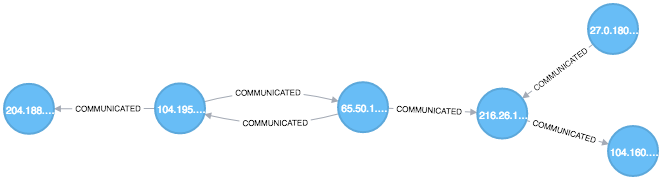
\includegraphics[width=0.75\textwidth]{gh0stRATgraph.png}
    \caption{Graph of IP addresses, visualized in Neo4j. Neo4j only handles directional relations, however, the analyses have been performed on a symmetric adjacency matrix, indicating an undirected graph.}
    \label{gh0stGraph}
\end{figure}

There are two similar data sets. The first set is based on 21,831 NetFlow records collected during the first months of 2017. In total, the data consist of 3,566 IP addresses where 204 of them have been identified as RAT controllers using packet inspection of responses from these controllers. A topographic view of the network can be seen in figure \ref{ip1}.

\begin{figure}[h!]
    \centering
    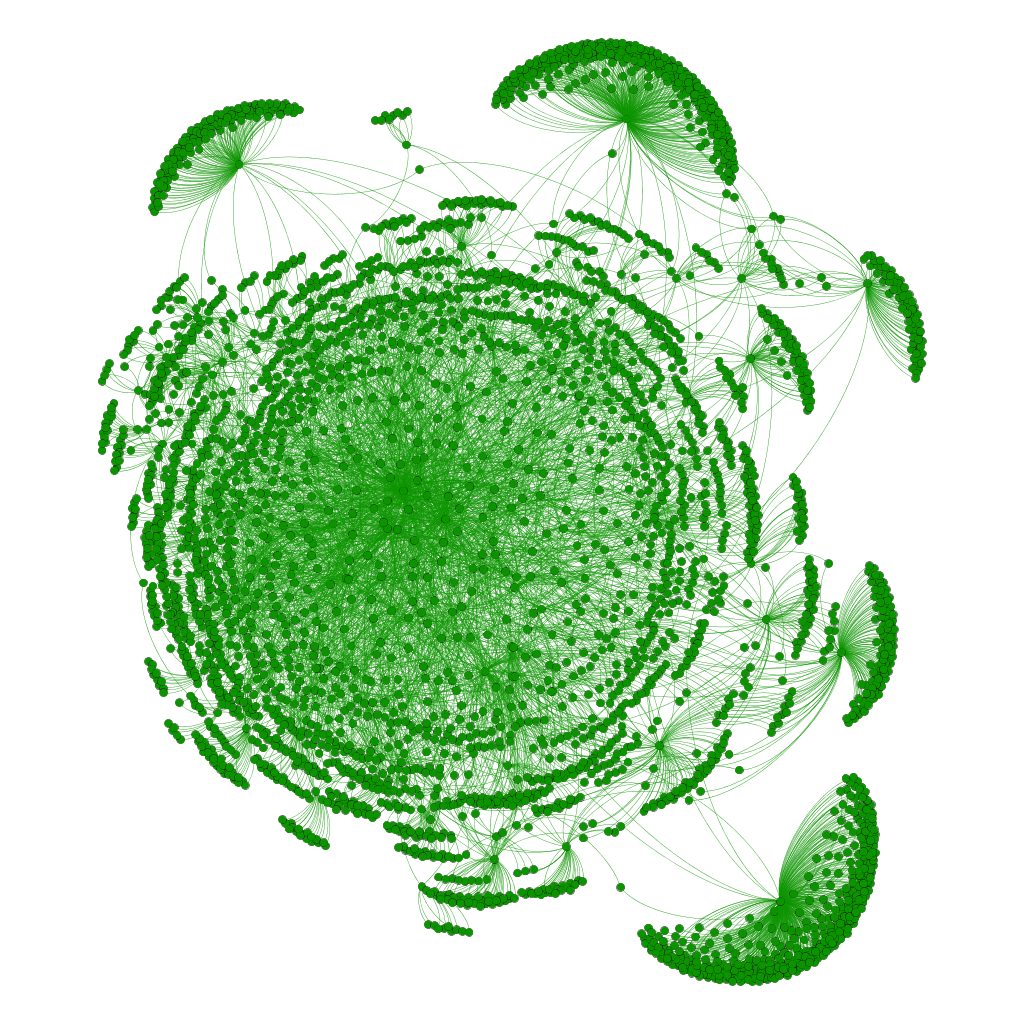
\includegraphics[width=0.5\textwidth]{GhostRATs.png}
    \caption{Graph of IP addresses, consisting of 3,566 nodes with 204 known RAT controllers. The graph is visualized using Gephi.}
    \label{ip1}
\end{figure}

The second data set consists of 103,202 NetFlow records collected during December 2016 to March 2017. This data set includes 10,091 IP addresses but is far more sparse with \textit{Gh0st}s, containing only 32 identified RAT controllers. 

In this case, the aim was to classify IP addresses, given the knowledge of only a few RAT controllers. As a consequence, we also aimed at identifying IP addresses that are incorrectly annotated as \textit{Non-gh0st}s. 

The classification has been performed by applying different similarity measures to the network. The applied similarity measures are the Dice coefficient, the Jaccard index, the cosine coefficient, the hub-promoting index and the hub-depressing index. These are all measures of structural equivalence and reflect the similarity based on the local structure, i.e. only the overlap of nearest neighbors.

Furthermore, the Local Path index and the Katz index were studied. Instead of simply studying the information of the nearest neighbors, they also account for more information about the topology. However, the two involve the parameter $\alpha$ that should be properly chosen. To chose it, a fraction of the dataset (20\%) was used to choose the best value of the parameter. 

The similarity was calculated for all nodes, given a small portion (1-5) of known Gh0st RAT controllers, henceforth referred to as reference nodes. Thus, the similarities for one node, in relation to the reference nodes, were simply taken as the sum. To classify the node, a threshold was then applied. If the similarity value exceeded the threshold, the node was classified as a RAT controller, i.e. a \textit{Gh0st}.

Once the classification was performed, the classifiers, using different similarity measures, were evaluated. The evaluation was based on the AUC of the precision recall curve and the F$_1$ score. AUC can be interpreted as a value of robustness of the similarity measure while F$_1$ represents the accuracy.

\subsection{Classification of Malicious IP Addresses \label{methodSVM}}
In this case, we have 102,540 IP addresses from the Recorded Future database. In the graph, the IP addresses are represented as nodes with relations referred to as ``RELATED TO''. The reason the relations have that specific label is because of the nature in which we do not know any more specific details about their co-occurrence. Furthermore, in the graph there are nodes related to malware, attack vectors\footnote{The path or means by which an attack is executed.} and cyber vulnerabilities. These have served as additional information which has been used as information about the neighboring IP addresses.

Recorded Future classifies the IP addresses by giving them a risk score, based on roughly 40 rules. There are 5 different risk classes
\begin{enumerate}
    \item None
    \item Unusual
    \item Suspicious
    \item Malicious
    \item Very Malicious
\end{enumerate}

The histogram of the classifications of the dataset is shown in \figref{hist}. We find the data to have an exponential distribution function, being extremely skewed to the left. Class 1 includes 60\% of the data, class 2 33\%, class 3 4\%, class 4 2.5\% and class 5 0.5\%. This introduces the problem of unbalanced data, discussed in \secref{unbalanced}. To deal with this issue, class weights were introduced such that an error from data in the minority class 5 was penalized higher than the error from data in the majority class 1. The weights were chosen to be inversely proportional to the number of samples in each class in the training set.

\begin{figure}[h!]
    \centering
    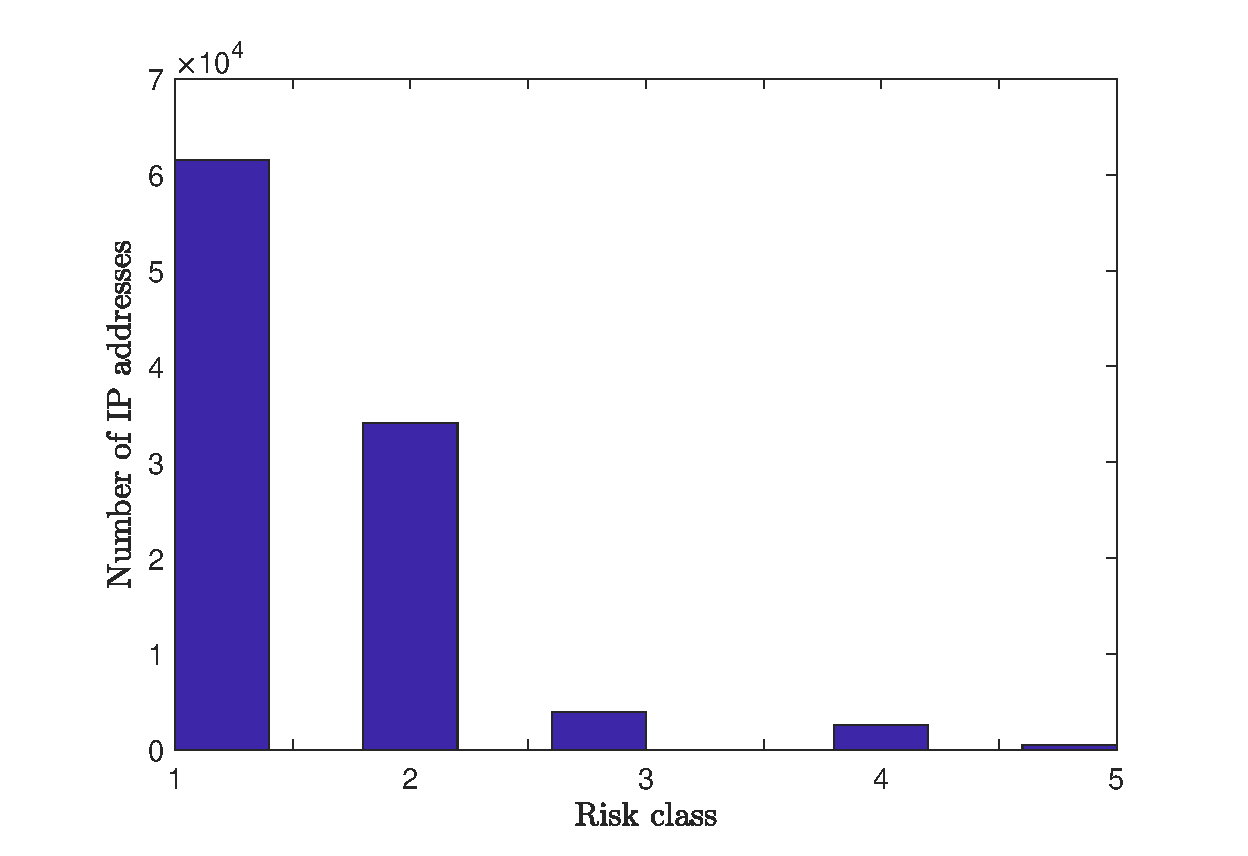
\includegraphics[width=0.6\textwidth]{dataHist.eps}
    \caption{Histogram of the IP classifications.}
    \label{hist}
\end{figure}

This case studies whether a graph approach with far less information might be enough to reconstruct Recorded Future's rule based classification. Removing any of their enriched data, we have simply used data found in the original reference. Thus, the following bold question is asked \textit{Is there a way of reconstructing Recorded Future's rule based classifier using a graph representation?} 

To classify the nodes, we have implemented a feature based node classifier. Using features based on topological information, predictions about their criticality was performed.

% Feature extraction
The term feature extraction refers to methods used for constructing node variables from the structure of the graph. These features were then used a input parameters for the classifier. Thus, the performance is highly dependent on the choice of features. In our case, the following features were used
\begin{itemize}
    \item PageRank based on the topology of IP addresses.
    \item Degree based on an undirected graph including only the IP addresses.
    \item Total number of hits in Recorded Future's data base.
    \item Number of unique malwares related to the nearest neighbors.
    \item Number of unique cyber vulnerabilities related to the nearest neighbors.
    \item Number of unique attack vectors related to the nearest neighbors.
\end{itemize}

The features can be divided into two categories. The first includes the PageRank and degree, only using the topology of the graph including only the IP addresses. The second category includes more information from Recorded Future's database, such as the number of hits, co-occurrences with malwares and so on. To study the impact of the different categories of features, classifications were performed including all of the features, only the topology features and finally the features including information regarding the number of hits, malwares, cyber vulnerabilities and attack vectors.

% Choice of classifier
In this case, a SVM classifier has been studied. Many researchers have used SVM for feature classification and found good results \citep{campbell2011,liu2012}. For instance, \citet{liu2012} showed promising results predicting links in a social network based on a SVM feature classifier. The fact that it was easily extended to a multi-class classifier was also an advantage. Moreover, it is easy to implement and it happens to deal with noise and outliers is a satisfactory fashion using the slack variable, introduced in \secref{svmTheory}.

Next, a kernel had to be chosen for the SVM. Due to the intermeshed nature of our data, the linear kernel was ruled out and the Radial Basis Function (RBF) kernel was chosen. According to \citet{Hsu10apractical}, the RBF kernel is a good first choice, since the RBF nonlinearly maps the data into a higher dimensional space. In addition, it has the advantage of including fewer parameters than the polynomial kernel implying a lower complexity.

After choosing the SVM classifier with a RBF kernel, the parameters $C$ and $\gamma$ had to properly be chosen. In order to do so, a grid search was performed. Various pairs of $C$ and $\gamma$ were tried and evaluated based on cross-validation accuracy of 10\% of the data. This was to avoid the pitfall of overfitting to the only dataset available. Once again in accordance with the recommendation of \citet{Hsu10apractical}, an exponentially growing sequence of parameters were studied where $C\in\{10^{-2},5\cdot10^{-2},10^{-1},5\cdot10^{-1},10^{0},...,10^{3}\}$ and $\gamma\in\{10^{-3},5\cdot10^{-3},10^{-2},5\cdot10^{-2},...,10^{2}\}$. The evaluation of the classifier was based on the accuracy, referring to the fraction of correct predictions in relation to Recorded Future's classifications. The set of parameters were chosen by maximizing the accuracy while making sure the predictions included all five classes. Since three different sub-cases were studied, each including a different set of features, the grid search was performed for each individual case. 

The SVM takes a matrix of features as input. As mentioned in \secref{scale}, it is preferable to rescale the feature vectors to avoid that some features are dominated by others. The rescaling was performed for each feature, in the range $[0,1]$, keeping the interrelation between elements in the feature vector. This is in accordance with the recommendation of \citet{Hsu10apractical}.

% Cross-validation including split into training and test set
To validate the classifiers, a 10-fold cross-validation was applied with 50 repetitions, in order to get a good statistical foundation.

Because of the skewness of the dataset, a pseudorandom classifier, based on a uniform distribution, was also implemented.  The results from it was then used in order to evaluate the SVM results. 

\subsection{Cyber Attacks}\label{cyberattacks}
Recorded Future's database contain entities that represents an event called cyberattack. The cyberattack entity is based on information found on the open internet as well as the dark/deep web. The entity may contain information such as the time when the attack is believed to have taken place, the author of the source of information, possible attackers and target as well as vulnerabilities and methods used to mention a few.

The whole set of cyberattack events is quite large. To predict future cyber attacks by the method of link prediction bipartite graphs described in \secref{sec:plp} we used only a subset of the cyber attack entities containing only the entities with a mention of an attacker and a target. The size of the subset containing all such references was 1435073. The number of cyber attacks that was indexed as taken place last month was 36297 which indicates how fast the subset we are using for analysis is growing.

The cyber attacks in the data set was represented in bipartite graph with the two adjacent sets being attackers and targets. It is worth mentioning that there are several cases where an entity appears as an attacker in one cyber attack and later as a target in another cyber attack. This goes against the definition of the bipartite graph. The solution was to create two different vertices representing in one case an attacker and in the other a target for such entities. The number of references for each attacker-target pair was used as the weight of the edge between the attacker and the target of the attack in the graph.

The running time of the PLP-algorithm by \citet{plp}, described in section \secref{sec:plp} is O(m) with m being the size of the smallest of the two adjacent sets of nodes in the bipartite graph. The subset we used is containing XX unique attackers and YY unique targets. And hence the running time will be O(a) where a is the number of attackers.

Even if PLP is quite efficient the running time could be reduced even further if link prediction could be made with good accuracy using only the most recent cyber attacks. Therefore we we investigated how the number of prediction and the precision was affected by different of length of time periods used for prediction. We were also interested in finding out what can could be said about when a predicted attack will take place and therefore we also varied the length of the time period used for testing the predictions.

To get good statistical values we repeated each experiment 10 times by randomly picking a start date for the prediction data set. We then computed the average values together with the standard deviations.

To evaluate how well PLP was able to predict future cyber attacks we primarily used two values. 
\paragraph{AUC}\label{plp:auc}
We wanted to find out how often the predictive index was higher for attacks that existed in the test set than for predictive indexes for attacks that was not in the test set. We therefore measured the AUC as
$$
  AUC = \frac{A+0.5C}{n},
$$
where A is the number of times where the existing attacks had a higher index, C is the number of times the index was the same and $n$ is the number of comparisons. We see that if the existing attacks has a higher index in all comparisons the precision is 1, if all compared index is equal the precision is 0.5 and if the index was higher for all non-existing attacks the precision is 0.

\paragraph{Prediction Rate}\label{plp:predict_rate}
Since PLP only gives a predictive index for the candidate node pairs it is reasonable to evaluate how many of the attacks in the test set that was given prediction index. We computed the prediction rate simply as
$$
  \frac{p}{m},
$$
where $p$ is the number of attacks in the test set that was given an index by PLP and $m$ is the number of attacks with unique pairs of attackers and targets.

The algorithm is naturally limited by that it is not able to predict attacks where the attack-target pair exist in a attack already in the prediction set. The algorithm is not able to predict attacks involving attackers or targets not in existence in the prediction set. Based on this it is interesting to see how many of the attacks in the test set are attacks that consist of a attacker-target pair not already in the prediction set but with each of the attacker and target individually in the prediction set.



\newpage 


\chapter{Results}
In this chapter our 

\section{Graph Database}
% Power of graph databases
We are dealing with connected data, where choosing a graph database have two advantages according to \citet{robinson2013}: performance and flexibility. In a relational database, the join-intensive query performance deteriorates as the dataset gets larger while, with a graph database the performance remains relatively constant. This is due to the fact that a query is only localized to a fraction of the graph making the run time proportional to the size of the sub-graph related to the query rather than the overall graph containing all available data.

Furthermore, there is the aspect of flexibility. Graphs are naturally additive \cite{robinson2013} such that new sub-graphs can be added containing more nodes and edges and new relations can be introduced as the understanding of the dataset grows. This have a positive implication for the analysts that does not have to model the domain in exhaustive detail from the start but can add information as time progress. 

Thus, according to the motivation above, we expect to use Neo4j, which is a cloud based graph database supporting some basic analysis through their query language Cypher.

\section{Gh0st RAT}
% In discussion - what similarity measure was the most appropriate to use in our case?

\begin{figure}[h!]
    \centering
    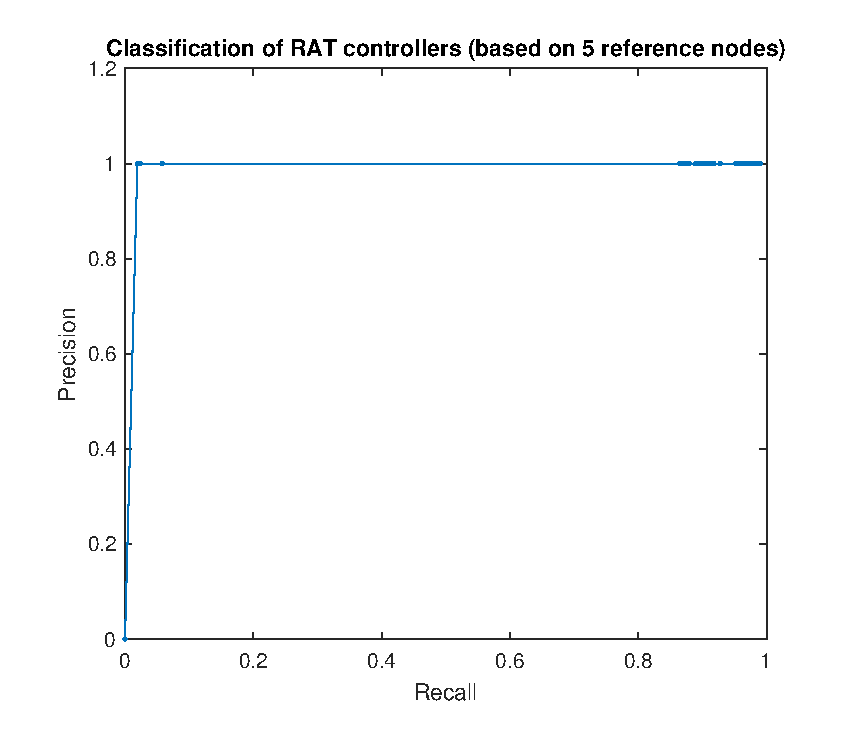
\includegraphics[width=0.4\textwidth]{precisionRecallRAT.eps}
    \caption{Caption}
    \label{fig:my_label}
\end{figure}

\begin{figure}[h!]
    \centering
    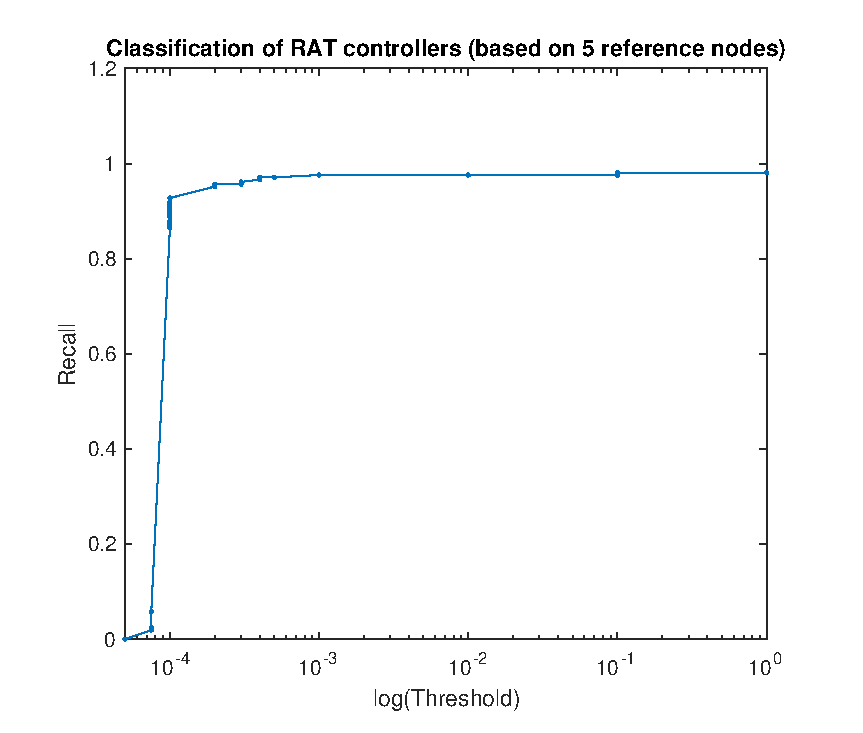
\includegraphics[width=0.4\textwidth]{recallThresholdRAT.eps}
    \caption{Caption}
    \label{fig:my_label}
\end{figure}

\section{Classification of malicious IP addresses}

\section{Redundancies}

\section{Target and Attackers}





\begin{comment}
\section{Multidimensional graph}
We expect a data representation where we have a multipartitioned graph, meaning there is a number of different nodes representing different kinds of entities with multiple edges, representing different relations, in between the nodes. Hence, we will then obtain a multidimensional network. 

\section{Analysis}
As far as the analysis goes, we expect to perform clustering to identify communities and link analysis to find different paths between two nodes. The latter can easily be queried in Neo4j and is expected to contribute a great deal solving the different questions. We also expect to use of some statistical tools such as average node degree, degree distribution and network diameter.
\end{comment}

\chapter{Discussion}
In this chapter, a discussion is held about the graph representation as well as the three studied cases. The chapter is concluded with a brief discussion about future work.

\section{Extracting data from docuement database}
% Power of graph databases
We are dealing with connected data, where choosing a graph database have two advantages according to \citet{robinson2013}: performance and flexibility. In a relational database, the join-intensive query performance deteriorates as the dataset gets larger while, with a graph database the performance remains relatively constant. This is due to the fact that a query is only localized to a fraction of the graph making the run time proportional to the size of the sub-graph related to the query rather than the overall graph containing all available data.

Furthermore, there is the aspect of flexibility. Graphs are naturally additive \cite{robinson2013} such that new sub-graphs can be added containing more nodes and edges and new relations can be introduced as the understanding of the dataset grows. This have a positive implication for the analysts that does not have to model the domain in exhaustive detail from the start but can add information as time progress.


\section{Gh0st RAT Controllers}
% In discussion - what similarity measure was the most appropriate to use in our case?
Based on the results, the simple local indices perform very well on both of the two data sets. The F$_1$ score seem to increase with the number of reference nodes which seems reasonable since the the change of a high recall is correlated with having reference nodes well distributed in the network. The change of getting a good distribution gets higher the more reference nodes. 

It may be surprising that the classifier based on local similarity generates such good results. However, it has to do with the graph itself, and how it is modelled. One reason for the good results is the the density of the graph. The local similarity measures are based solely on the nearest neighbors implying that all of the RAT controllers must share one common neighbor with one of the known RAT controller from the start in order to be found. If one (unclassified) RAT controller is positioned in the periphery of the network, far away from the reference nodes, that will never be properly classified. Hence, using local similarity measures for classification is highly dependent of the density of the graph and/or a good distribution of the reference nodes in the graph. 

The high density of the graph can also explain the fact why the Local Path index and the Katz index does not perform as well as the local index. Including more neighbors to account for the similarity makes the method sensitive to finding the best threshold. If the threshold is badly chosen, it will either result in bad precision or bad recall resulting in a poor accuracy.

% Falsely annotated IP addresses
In the first dataset, three IP addresses annotated as \textit{Non-ghost}s were classified as \textit{Gh0st} in the majority of the cases. There is reason to believe those IP addresses are falsely annotated and are in fact RAT controllers. This could be confirmed by one of the analysts at Recorded Future.

If we handle the three falsely annotated IP addresses as RAT controllers, we find that we get an accuracy of 100\% when including 3 or more reference nodes trying to classify nodes using similarity. 

To conclude, we find that the local indices perform very well in this particular case of classifying IP addresses based on a graph modelled from NetFlow data. They are robust in the sense that they are not sensitive to the choice of threshold, which can be set to zero and still output good performance. The five different local indices that were tried does not vary much in performance and thus any of them can be recommended to be used. This method could be used both for binary classification of unknown IP addresses where only a few are known to belong to a certain class. Furthermore, it can be used to identify falsely annotated IP addresses. 

\section{Classification of malicious IP addresses}
All of the three SVM models perform far better classification than a random classifier. The model with 4 features performs better than the one using only 2 nodes, however, the best one is the combination, when all 6 features are used. 

The SVM classifier seems to have a bias towards the lower risk classes, for all of the three SVMs. This may very well have to do with the dataset being extremely skewed. We see that all of the three SVMs perform far less higher classifications than the random classifier and more lower classifications than the random classifier.

% Skewed dataset (Theory: Imbalanced datasets http://www.sciencedirect.com/science/article/pii/S0020025514003272)

% A lot of noise in the dataset
One reason for the low result may very well have to do with the noise in the dataset. In this context, noise is referred to as IP addresses that by Recorded Future's rule based system would have been classified with a high risk class however, have an exception. One such example is Google's DNS server, which have been set to a risk class of 1 since it is not regarded to be a malicious source. 

It is hard to quantify the amount of noise present in the data, however it is only reasonable to believe it has an impact on the results. We can thus derive some of the poor classifications to noise. 

Although an accuracy of 75\% can be argued to be rather good, it is not by far good enough serve as an independent classification system of Recorded Future and we can recognize the fact that we were not able to reconstruct Recorded Future's current classification system. However, with some modifications, where more features are included, we believe the performance can be increased. Even though it may be hard to reach an accuracy sufficiently high to accept it as a valid classification system at Recorded Future, this kind of methods could serve as an learning tool, leading to many important insights for Recorded Future. Not only could it tell them a lot about their classification system today, but also drive insights towards what kind of features or information that are the most important when classifying IP addresses. In that way, new rules could be added of perhaps old ones made less significant. 

% How can the classifier be improved?
It should be mentioned that the aim was to include two more features, namely the betweenness centrality and the closeness centrality. The calculations of the centrality measures were started in Cypher in Neo4j, however, the large amount of data resulted in a very long runtime (> one week using the Cypher-shell), and thus the conclusion that the network was too big for these measures was drawn. The betweenness and closeness centrality might have contributed to better predictions but were excluded from our model.

\section{Prediction of Future Cyber Attacks}
% Incorrectness of results due to incorrectness in DB
% Running time
% Limitations because of earlier attacks and new actors
% Maximum prediction rate
% Length of train periods

Before discussing the results of the PLP algorithm on the cyber attack data set it is worth mentioning that the predictions made does not necessarily indicate that attack is likely to happen. Because the dataset is based on mentions on the internet of cyber attacks, what is being predicted is the future possibility of mentions of cyber attacks such that it is recorded and added to the Recorded Future Database. Such recordings might be incorrect since NLP together with other algorithms is used to harvest the information from the sources.

However, the accuracy of the predictions is for all time periods tested impressing. The prediction rate is naturally limited by that it is not possible to predict attacks involving actors (targets or attackers) not already in the data set used for prediction. There is also a limit because the algorithm does not give a predictive index for attacks that consists of the same set of actors that has previously been involved together in a previous attack. The maximum prediction rate possible due to the factors just discussed varied between 60\%-70\%. With these limiting factors in mind, a prediction rate of 20\%-25\% together with the high accuracy of the predictions is good enough for the algorithm to be useful in the applied work of predicting cyber attacks.

The most likely reason for the prediction rate not being higher is probably because graph representing the data set contains a lot of isolated sub graphs that limits the algorithm ability. Then there is of course the factor that threat actors act unpredictably which is the reason why companies trying to counter cyber attacks invests a lot of time and resources on intelligence work.

What is most interesting is that ~20\% of cyber attacks can be predicted just by using the available topological information in the bipartite graph without using any domain knowledge.

To further improve the algorithm it would be interesting to see if it would be possible to predict new attacks that has already happened once before.

In many cases the interest of predicting future cyber attacks stem from the need to prepare and prevent such attack. The name of the attacker might then only be of secondary interest. The primary interest is to find out what methods might be used and what vulnerabilities might be exploited. With this in mind the bipartite graph could be constructed by a set of attacker profiles and target name instead of attacker name and target name. The profiling could be based on what vulnerabilities and methods the attacker has previously used, together wish other domain specific information. This would reduce the number of vertices in the graph and make it denser. It would also enable to predict attacks with attackers not already in the database if the future attacker fits a profile in the database.


\section{Future Work}
This report has only covered a small part of interesting methods based on graph theory that might be of interest to apply to the cyber threat intelligence domain. Thus, we now present some interesting ideas that was stumbled upon without having the resources to try them out. 

In the Gh0st RAT controller case, structural equivalence was used for classification of nodes. However, there is another similarity called regular equivalence that takes the position of the node into consideration. Thus, two nodes are regularly equivalent if they are equally related to equivalent others. Although structural equivalence measure might have been enough for the RAT controller case, there are many different areas where regular similarity would suit better. However, the disadvantage of regular equivalence it that it implies an iterative or recursive nature since the similarity between the neighborhoods of the nodes has to be known before the similarity of the nodes themselves can be computed \cite{leicht2006}. Thus, the regular equivalence involves a higher complexity than many of the structural equivalence measures, however it could lead to new insights. 

In this study, we have selected only a few features for our classifier. We have also limited our research to only account for a very small amount of all the information available in Recorded Future's database. Thus, a natural extension of this research may be to include other and more features in the classification model. Such studies could lead to more insights about Recorded Future's current classification system.

The PLP was only evaluated on the data set of cyber attacks but might as well be applicable to other data set that can be naturally represented by a bipartite graph. One example is terror attacks and another is terror financing, but any other scenario might also be of interest.

Another interesting idea is to mine the graph for often occurring sub-structures. This might be done with a more exploratory interest in mind. One algorithm for such a purpose is the AProximate Graph Mining (APGM) developed by \citet{Jia2011}, that looks for often occurring structures but accounts for noise and perturbations in the original data. This can be of high interest for Recorded Future because of the uncertain nature of the data, covered in \secref{dataset}.


\chapter{Conclusions}

% 


\newpage
\printbibliography[heading=bibintoc]

%%%%%%%%%%%%%%%%%%%%%%%%%%%%%%%%%%%%%%%%%%%%%%%%%%%%%%%%%%%%%%%%
% Bilaga
\appendix
\renewcommand{\appendixtocname}{Appendix}
\addappheadtotoc
\numberwithin{equation}{section}
\chapter{PLP algorithm}\label{ap:plp}
The PLP algorithm such as it was implemnted in this work and developed by \citet{plp}.


\makeatletter
\def\BState{\State\hskip-\ALG@thistlm}
\makeatother

\begin{algorithm}
\caption{PLP algorithm}

\begin{algorithmic}

\State $ \textbf{U} \gets \text{Set of vertices of type A}$
\State $ \textbf{V} \gets \text{Set of vertices of type B}$
\State $ \textbf{E} \gets \text{Set of edges}$
\State $ \textbf{G} \gets \text{Graph }\textbf{G}=(\textbf{U},\textbf{V},\textbf{E})$

\State /* Construct the set of all patterns */

\State $ \textbf{E}_u \gets \emptyset$
\For{each node in B in \textbf{U}}
    \For{each node x in \textbf{N}(B)}
        \For{each node in C in \textbf{N}(x)}
            \State $\textbf{E}_u \gets \textbf{E}_u \cup \{(B,C)\}$
        \EndFor
    \EndFor
\EndFor

\State /* Calculate the weight of each pattern */

\For{each edge (B,C) in $\textbf{E}_u$}
    \State Calculate the weight for pattern (B,C)
\EndFor

\State /* Calculate the connectivity of CNPs */

\For{each node B in projected graph $\textbf{G}_u$}
    \For{each neighbor C of B in projected graph $\textbf{G}_u$}
        \For{each node x linked with C in \textbf{G}}
            \If{(B,x) $\notin$ \textbf{E}}
                \State S(B,x) = S(B,x) + w(B,C)
            \EndIf
        \EndFor
    \EndFor
\EndFor

\State /* Output the connectivity of the CNPs in matrix S.

\end{algorithmic}
\end{algorithm}


\end{document}

